% Euclidean Handout Number sixteen
\documentclass{tufte-handout}

%\geometry{showframe}% for debugging purposes -- displays the margins

%%%% Packages to make things pretty
\usepackage{amsmath,amsthm}
\usepackage{booktabs}
\usepackage{graphicx}
\setkeys{Gin}{width=\linewidth,totalheight=\textheight,keepaspectratio}
\graphicspath{{graphics/}}
\usepackage{units}
\usepackage{fancyvrb}
\fvset{fontsize=\normalsize}
\usepackage{multicol}
\usepackage{pdfpages}

%%%% Theorem Environments
\theoremstyle{definition}
\swapnumbers
\newtheorem{problem}{Problem}[section]
\newtheorem{conjecture}[problem]{Conjecture}
\newtheorem*{definition}{Definition}
\newtheorem*{theorem}{Theorem}
\newtheorem{question}[problem]{Question}
\newtheorem{challenge}[problem]{Challenge}
\newtheorem*{postulate}{Postulate}

%%%%%

\title{Euclidean Geometry:\\An Introduction to Mathematical Work}
\author[]{Math 3600}
\date{Spring 2020}

\begin{document}

\maketitle

\begin{marginfigure}
    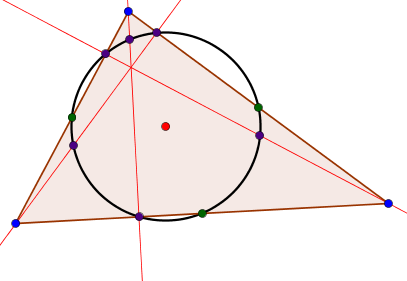
\includegraphics{NPC}
\end{marginfigure}

\setcounter{section}{16}
\section{The Regular Pentagon Rides Again}


The next three tasks concern the following construction template for inscribing a regular pentagon in a circle. 

\vspace{.5in}

Given a circle with center $O$,
\begin{compactenum}
\item Draw any line through $O$; get $A$ and $B$.
\item Draw $\odot AB$.
\item Draw $\odot BA$, get $C$ as intersection of last two circles.
\item Draw line $OC$, get $D$ between $O$, $C$ as intersection with given circle.
\item Draw $\odot DO$, get $E, F$ as intersections with given circle.
\item Draw $EF$, get $G$ as intersection with $OC$.
\item Draw circle $\odot GA$, get point $H$ as intersection with ray $DO$.
\item Draw circle $\odot A(OH)$, get points $I, J$ as intersections with given circle.
\item Draw circle $\odot B(IJ)$, get points $K, L$ as intersections with the given circle.
\item (five steps) Draw segments $BK, KJ, JI, IL, LB$.
\end{compactenum}
\marginnote[-60pt]{The notation $\odot A(BC)$ means a circle with center $A$ and radius congruent to segment $BC$.}

\vspace{.5in}

\begin{conjecture}\label{conj:pentagon-1}
Triangle $OAI$ is isosceles and its base angles are twice the angle at $O$.
\end{conjecture}

\begin{conjecture}\label{conj:pentagon-2}
Triangle $BJI$ is isosceles and its base angles are twice the angle at $B$.
\end{conjecture}

\begin{conjecture}\label{conj:pentagon-3}
Show that $BKJIL$ is a regular pentagon.
\end{conjecture}

\vfill
\end{document}

%sagemathcloud={"zoom_width":100}